\documentclass{article}
\usepackage{pgfplots}
\title{KEEL: ROC output}
\begin{document}
\maketitle
\pagebreak[4]
\hfill \break
Section one: TEST FILE
\hfill \break
\hfill \break
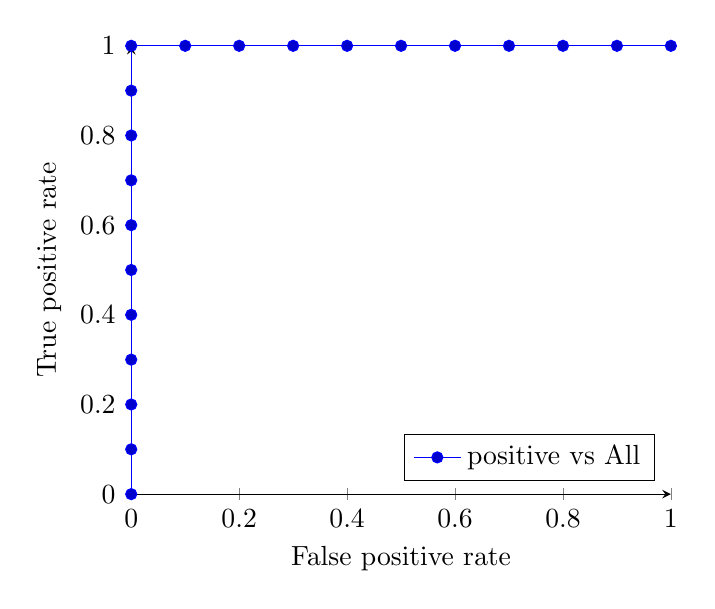
\begin{tikzpicture}
\begin{axis} [xlabel=False positive rate,
ylabel=True positive rate,axis x line=bottom,
axis y line=left, legend pos=south east]
\addplot coordinates { (0,0)(0.0,0.1)(0.0,0.2)(0.0,0.30000000000000004)(0.0,0.4)(0.0,0.5)(0.0,0.6)(0.0,0.7)(0.0,0.7999999999999999)(0.0,0.8999999999999999)(0.0,0.9999999999999999)(0.1,0.9999999999999999)(0.2,0.9999999999999999)(0.30000000000000004,0.9999999999999999)(0.4,0.9999999999999999)(0.5,0.9999999999999999)(0.6,0.9999999999999999)(0.7,0.9999999999999999)(0.7999999999999999,0.9999999999999999)(0.8999999999999999,0.9999999999999999)(0.9999999999999999,0.9999999999999999)};\addlegendentry{positive vs All}
\end{axis}
\end{tikzpicture}\hfill \break
\hfill \break
 Area Under Curve (AUC):0.9999999999999998
\hfill \break
\hfill \break
\end{document}